%% ****** Start of file apstemplate.tex ****** %
%%
%%
%%   This file is part of the APS files in the REVTeX 4.2 distribution.
%%   Version 4.2a of REVTeX, January, 2015
%%
%%
%%   Copyright (c) 2015 The American Physical Society.
%%
%%   See the REVTeX 4 README file for restrictions and more information.
%%
%
% This is a template for producing manuscripts for use with REVTEX 4.2
% Copy this file to another name and then work on that file.
% That way, you always have this original template file to use.
%
% Group addresses by affiliation; use superscriptaddress for long
% author lists, or if there are many overlapping affiliations.
% For Phys. Rev. appearance, change preprint to twocolumn.
% Choose pra, prb, prc, prd, pre, prl, prstab, prstper, or rmp for journal
%  Add 'draft' option to mark overfull boxes with black boxes
%  Add 'showkeys' option to make keywords appear
%\documentclass[aps,prfluids,preprint,superscriptaddress]{revtex4-2}
%\documentclass[aps,prl,preprint,superscriptaddress]{revtex4-2}
\documentclass[aps,prfluids,reprint,superscriptaddress]{revtex4-2}

\usepackage{graphicx}
\usepackage[hypertexnames=false,
pdfstartview=FitH,
breaklinks=true,
bookmarks=true,
bookmarksopen=true,
bookmarksnumbered=true]{hyperref}
\urlstyle{same}
\hypersetup{
	colorlinks = true,
	linkcolor  = blue,
	urlcolor   = blue,
	citecolor  = blue,
}
\setlength{\parskip}{0cm plus4mm minus2mm}
\setlength{\bibsep}{-1.45pt}

\usepackage{natbib}

%user defined commands
\newcommand{\h}[1]{\textbf{\textit{#1}}}
\newcommand{\ii}[1]{\text{#1}}
\newcommand{\noi}{\noindent}
\newcommand{\nn}{\nonumber}
\newcommand{\overbar}[1]{\mkern 1.5mu\overline{\mkern-2mu#1\mkern-2mu}\mkern 1.5mu}
%for roman numeral
\newcommand{\RN}[1]{%
	\textup{\uppercase\expandafter{\romannumeral#1}}%
}
\newcommand{\Rn}[1]{%
	\textup{\expandafter{\romannumeral#1}}%
}
\renewcommand{\textrm}{\rm}
\usepackage{siunitx} % JCBdM: I add this to avoid incompatibility
\usepackage{bm} % Bold in math mode
\usepackage{amsmath} %extra math packages
\usepackage{amssymb} %for math symbols
\usepackage{physics} %for partial differential equations
\DeclareDocumentCommand\dpdv{}{\displaystyle\partialderivative}
\usepackage{multirow}
\usepackage{cancel}
\usepackage{scalerel} %change size of subscripts
\usepackage{soul,color}
\usepackage{ulem}
\usepackage{xcolor}
\usepackage{hhtensor}

\newcommand{\Wietze}[1]{\textcolor{teal}{#1}}
\newcommand{\red}[1]{\textcolor{red}{#1}}

\DeclareRobustCommand{\hly}[1]{{\sethlcolor{yellow}\hl{#1}}}
\DeclareRobustCommand{\hlr}[1]{{\sethlcolor{pink}\hl{#1}}}


\newcommand{\mref}[1]{{\hypersetup{linkcolor=black}\ref{#1}}}
\newcommand{\meqref}[1]{{\hypersetup{linkcolor=black}\eqref{#1}}}


%tikz
\usepackage{pgfplots, tikz}
\usetikzlibrary{3d}
\usepackage{tikz-3dplot}
\pgfplotsset{compat=newest} 
\usetikzlibrary{shapes.geometric}
\usetikzlibrary{arrows.meta}
\usetikzlibrary{positioning}
\usepgfplotslibrary{external}
%\tikzexternalize[prefix=cache/]

\usepackage{flafter}
\usepackage{mdframed}
\usepackage{float}

\usepackage{xr}
\externaldocument{../mag_damp_prf}

\numberwithin{equation}{section}

\begin{document}
\section{Supplementary material: Derivation of the time independent induced electric potential for a two-layer system in a rectangular domain}
\label{supplA}

In this section, we derive the induced electric potential for a rectangular domain with four different electrical boundary conditions. The first has a trivial solution i.e. $\Psi_i|_{\Omega_i} = 0$. The rest of the case descriptions along with the boundary conditions are provided in Table\,\ref{tab:table_BC_cases}. Considering that the potential is non-zero when the boundary is insulating, we first derive $\Psi$ in a domain with all insulating walls (B.C 4). Cases B.C 2 and 3 are modifications of B.C 4. 

\begin{table}[H] %add [H] placement to break table across pages
	\caption{The electrical boundary and interface conditions of the three cases where we derive the induced electric potential $\Psi$.}
	\label{tab:table_BC_cases}
	\begin{ruledtabular}
		\begin{tabular}{llll}
			Case No. &  Case name & \multicolumn{2}{l}{Boundary conditions} 
			\\  \hline 
			2 & B.C 2 &
			\multirow{5}{*}{
				\begin{tikzpicture}
					\node at (0,0) {
						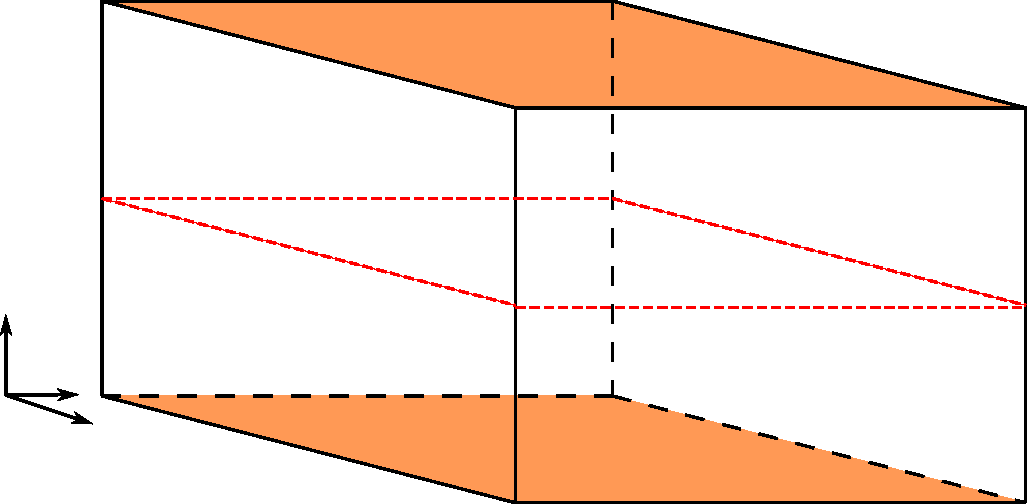
\includegraphics[width=0.3\textwidth]{figures/BC_case2.pdf}
					};
					\node (y) at(-2.1,-0.95) {$y$};
					\node (x) [above of=y, xshift=-0.2cm, yshift=-0.6cm] {$x$};
					\node (z) [above of=y, xshift=-0.55cm, yshift=-0.2cm] {$z$};
				\end{tikzpicture}
			}
			& 
			\\
			& & & $\partial_x \widehat\Psi\bigl|_{x=\pm 0.5L_x} = \partial_y\phi_i B_z$, 
			\\
			& & & $\partial_y \widehat\Psi\bigl|_{y=\pm 0.5L_y}= -\partial_x\phi_i B_z$,
			\\
			& & & $ \widehat\Psi\bigl|_{z=h_1}=\widehat\Psi\bigl|_{z=-h_2}=0$
			\\
			& & &
			\\[22pt] \hline
			% 		
			3 &	 B.C 3 &
			\multirow{5}{*}{
				\begin{tikzpicture}
					\node at (0,0) {
						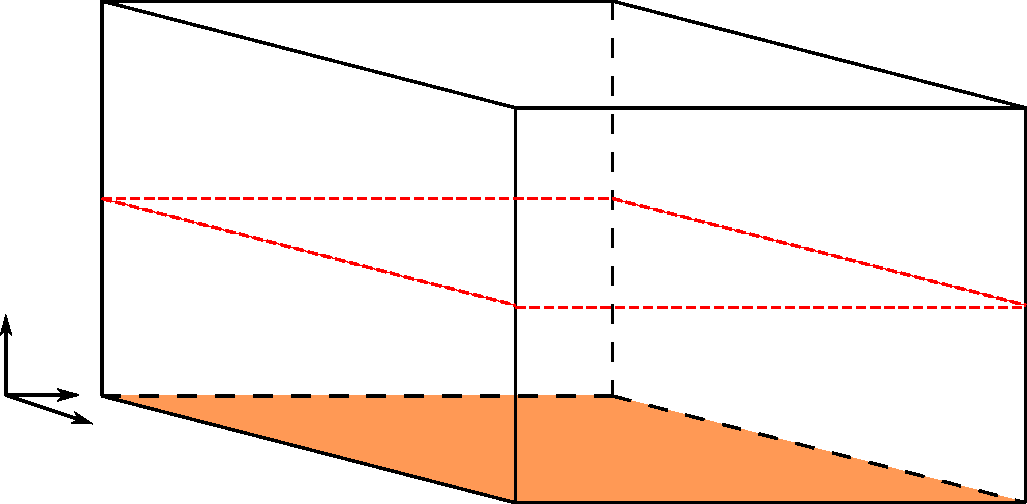
\includegraphics[width=0.3\textwidth]{figures/BC_case3.pdf}
					};
					\node (y) at(-2.1,-0.95) {$y$};
					\node (x) [above of=y, xshift=-0.2cm, yshift=-0.6cm] {$x$};
					\node (z) [above of=y, xshift=-0.55cm, yshift=-0.2cm] {$z$};
				\end{tikzpicture}
			}
			& 
			\\
			& & & $\widehat\Psi\bigl|_{x=\pm 0.5L_x}=0$, 
			\\
			& & & $\partial_y \widehat\Psi\bigl|_{y=\pm 0.5L_y}= -\partial_x\phi_i B_z$,
			\\
			& & & $\partial_z\widehat\Psi\bigl|_{z=h_1}=\partial_z\widehat\Psi\bigl|_{z=-h_2}=0$
			\\
			& & &
			\\[22pt] \hline
			
			4
			& B.C 4 &
			\multirow{5}{*}{
				\begin{tikzpicture}
					\node at (0,0) {
						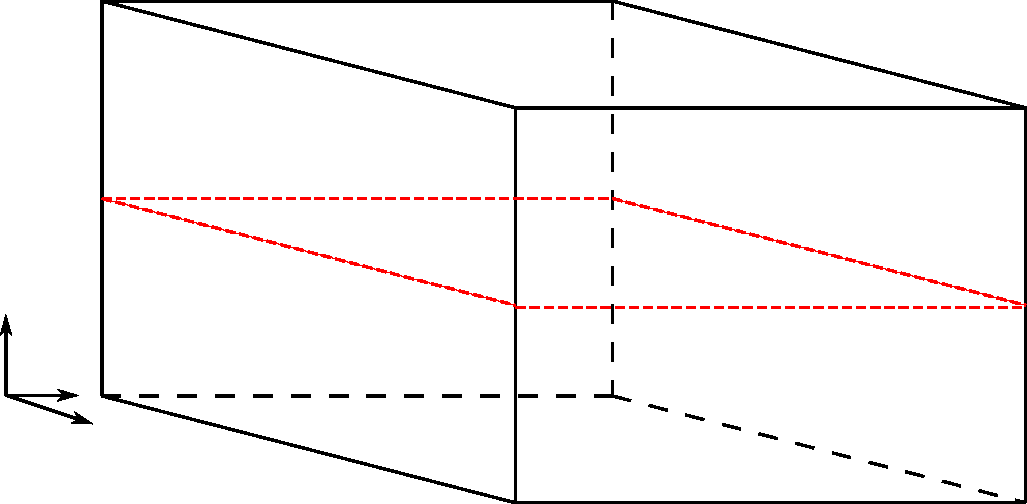
\includegraphics[width=0.3\textwidth]{figures/BC_case4.pdf}
					};
					\node (y) at(-2.1,-0.95) {$y$};
					\node (x) [above of=y, xshift=-0.2cm, yshift=-0.6cm] {$x$};
					\node (z) [above of=y, xshift=-0.55cm, yshift=-0.2cm] {$z$};
				\end{tikzpicture}
			}
			&
			\\
			& & & $\partial_x \widehat\Psi\bigl|_{x=\pm 0.5L_x} = \partial_y\phi_i B_z$, 
			\\
			& & & $\partial_y \widehat\Psi\bigl|_{y=\pm 0.5L_y}= -\partial_x\phi_i B_z$,
			\\ 
			& & & $ \partial_z\widehat\Psi\bigl|_{z=h_1}=\partial_z\widehat\Psi\bigl|_{z=-h_2}=0$
			\\
			& & &
			\\[22pt]
		\end{tabular}
	\end{ruledtabular}
\end{table}

\noi From Eq.\,\meqref{eq:laplacian_psi} in the main article, the Laplace equation for the induced electric potential can be expanded to
\begin{gather}
	\pdv[2]{\widehat{\Psi}_i}{x} + \pdv[2]{\widehat{\Psi}_i}{y}
	+ \pdv[2]{\widehat{\Psi}_i}{z}= 0 ,
\end{gather}
for given fluid layer $i=1,2$. We first solve for $\Psi_i(m,n) = A(x) \: B(y) \: C(z) \: H$, where $A$, $B$, $C$ and $H$ are functions with respect to $x$, $y$, $z$ and the interface amplitude accordingly
\begin{equation}
	\dfrac{1}{A} \dpdv[2]{A}{x}  + \dfrac{1}{B} \dpdv[2]{B}{y} 
	+ \dfrac{1}{C} \dpdv[2]{C}{z} = 0.
	\label{eq:laplace_ABC}
\end{equation}
Introducing constants $\xi_x$, $\xi_y$ and $\xi_z$ such that
\begin{equation}
	\xi_x^2 + \xi_y^2 + (-\xi_z^2) = 0 .
\end{equation}
At first glance from the given boundary conditions for B.C 4 in Table\,\ref{tab:table_BC_cases}, there is no straightforward way to solve the above Laplace equation using separation of variables, mainly due to the presence of non-zero boundary conditions in the $x$- and $y$-normal walls. This causes two of the constants to show exponential behavior in the solution, instead of the traditional system made out of one exponential and two oscillatory functions. Because the total sum of the balance must be zero, two of the constants need to have the opposite sign of the third. As a solution to this problem, the problem is to be divided into two constituent parts:
\begin{subequations}
	\begin{align}
	\RN{1} : \xi_x^2 + (-\xi_y^2) + (-\xi_z^2) = 0,
	\label{eq:laplace_m} 
	\\
	\RN{2} : (-\xi_x^2) + \xi_y^2 + (-\xi_z^2) = 0,
	\label{eq:laplace_n} 
	\end{align}
\end{subequations}
with Eqs.\,(\ref{eq:laplace_m} and \ref{eq:laplace_n}) solve the Laplace equation \eqref{eq:laplace_ABC} in a system with the following boundary conditions:
\begin{subequations}
	\begin{align}
		\RN{1} : \partial_x \widehat\Psi\bigl|_{x=\pm 0.5L_x} = \partial_y\phi_i B_z,\;
		\partial_y \widehat\Psi\bigl|_{y=\pm 0.5L_y}= 0, \;
		\partial_z\widehat\Psi\bigl|_{z=h_1}=\partial_z\widehat\Psi\bigl|_{z=-h_2}=0
		\label{eq:bc_m} 
		\\
		\RN{2} : \partial_x \widehat\Psi\bigl|_{x=\pm 0.5L_x} = 0, \;
		\partial_y \widehat\Psi\bigl|_{y=\pm 0.5L_y}= -\partial_x\phi_i B_z,\;
		\partial_z\widehat\Psi\bigl|_{z=h_1}=\partial_z\widehat\Psi\bigl|_{z=-h_2}=0
		\label{eq:bc_n} 
	\end{align}
\end{subequations}
We first solve for system \RN{1} considering the boundary conditions at $x=-0.5L_x$ and $x=0.5L_x$:
\begin{equation}
\pdv{\widehat\Psi_i}{x}\Bigl|_{x=-0.5L_x,0.5L_x} = \pdv{A}{x}\bigl(-0.5L_x,0.5L_x\bigr)B(y)C(z) = \pdv{\widehat\phi_i}{y}B_z\Bigl|_{x=-0.5L_x,0.5L_x}.
\end{equation}
The term $A(x)$ can be written as a sum of hyperbolic functions
\begin{equation}
	A(x) = A_{1x}\cosh{[\xi_x x]} + A_{2x}\sinh{[\xi_x x]},
\end{equation}
and at $x=-0.5L_x$:
\begin{align}
	\pdv{A}{y}\biggl|_{x=-0.5L_x} &= A_{1x}\xi_x\sinh{[-\xi_xL_x/2]}
	+ A_{2x}\xi_x\cosh{[-\xi_xL_x/2]},
	\\
	& = -\frac{n\pi}{L_y}\sin{\left[\frac{n\pi}{L_y}(y+0.5L_y)\right]} \cos{[0]},
\intertext{whereas at $x=0.5L_x$:}
	\pdv{A}{y}\biggl|_{x=0.5L_x} &= A_{1x}\xi_x\sinh{[\xi_xL_x/2]}
	+ A_{2x}\xi_x\cosh{[\xi_xL_x/2]},
	\\
	& = -\frac{n\pi}{L_y}\sin{\left[\frac{n\pi}{L_y}(y+0.5L_y)\right]} \cos{[m\pi]}.
\end{align}
When $m$ is odd,
\begin{equation}
2A_{2x}\xi_x\cosh{[\xi_xL_x/2]} = 0, \quad \therefore A_{2x} = 0 \Longrightarrow A(x) = A_{1x} \cosh{[\xi_x x]},
\end{equation}
and when $m$ is even,
\begin{equation}
-2A_{1x}\xi_x\sinh{[\xi_xL_x/2]} = 0, \quad \therefore A_{1x}=0 \Longrightarrow A(x) = A_{2x} \sinh{[\xi_x x]}.
\end{equation}
Therefore,
\begin{equation}
	A(x) = 
	A_{1x} \frac{1-(-1)^m}{2\sech{[\xi_x x]}} + A_{2x} \frac{1+(-1)^m}{2\csch{[\xi_x x]}}.
\end{equation}
At the $y$-normal walls,
\begin{equation}
	\pdv{B}{x} \: (-0.5L_y,0.5L_y) = 0,
\end{equation}
and therefore,
\begin{equation}
	B(y) = \sum_{a=0}^{\infty}
	B_{y} \cos{\biggl[ \frac{a\pi}{L_y}\Bigl(y + \frac{L_y}{2} \Bigr)\biggr]} .
\end{equation}
The boundary conditions at the top and bottom wall are
\begin{equation}
	\pdv{C_1}{z}\bigl(h_1\bigr) = 0,
	\quad
	\pdv{C_2}{z}\bigl(-h_2\bigr) = 0.
\end{equation}
leading to,
\begin{equation}
	C_i(z) = \sum_{b=0}^{\infty}
	 C_{z} \cos{\biggl[ \frac{b\pi}{h_i}\bigl(z + (-1)^i h_i\bigr)\biggr]},
	\qquad \{i=1,2\}.
\end{equation}
Combining the coefficients such that
\begin{equation}
	\left(A_{1x} \frac{1-(-1)^m}{2} + A_{2x} \frac{1+(-1)^m}{2}\right)
	B_y\: C_z = A_{ab},
\end{equation}
the solution for system \RN{1} is
\begin{equation}
	\Longrightarrow
	\sum_{a=0}^{\infty} \sum_{b=0}^{\infty}
	A_{ab} 
	\left(\frac{1-(-1)^m}{2\sech{[\xi_x x]}} + \frac{1+(-1)^m}{2\csch{[\xi_x x]}}
	\right)
	\cos{\biggl[ \frac{a\pi}{L_y}\biggl(y + \frac{L_y}{2}\biggr)\biggr]}
	\cos{\biggl[ \frac{b\pi}{h_i}\bigl(z+(-1)^ih_i\bigr)\biggr]} H.
\end{equation}
Similarly, the solution for system \RN{2} is
\begin{equation}
	\Longrightarrow
	\sum_{a=0}^{\infty} \sum_{b=0}^{\infty}
	B_{ab} 
	\left(\frac{1-(-1)^n}{2\sech{[\xi_y y]}} + \frac{1+(-1)^n}{2\csch{[\xi_y y]}}
	\right)
	\cos{\biggl[ \frac{a\pi}{L_x}\biggl(x + \frac{L_x}{2}\biggr)\biggr]}
	\cos{\biggl[ \frac{b\pi}{h_i}\bigl(z+(-1)^ih_i\bigr)\biggr]} H,
\end{equation}
where
\begin{equation}
	\xi_x = \pi\sqrt{
	\biggl(\frac{a}{L_y}\biggr)^2 + \biggl(\frac{b}{h_i}\biggr)^2
	}, \quad
	\xi_y = \pi\sqrt{
		\biggl(\frac{a}{L_x}\biggr)^2 + \biggl(\frac{b}{h_i}\biggr)^2
	}.
\end{equation}
Combining the solutions of system \RN{1} and \RN{2}, we get
\begin{align}
	\nn
	\Psi_i &= 
	\sum_{a=0}^{\infty} \sum_{b=0}^{\infty}
	A_{ab} 
	\left(\frac{1-(-1)^m}{2\sech{[\xi_x x]}} + \frac{1+(-1)^m}{2\csch{[\xi_x x]}}
	\right)
	\cos{\biggl[ \frac{a\pi}{L_y}\biggl(y + \frac{L_y}{2}\biggr)\biggr]}
	\cos{\biggl[ \frac{b\pi}{h_i}\bigl(z+(-1)^ih_i\bigr)\biggr]} H
	 \\
	 &+ 
	 \sum_{a=0}^{\infty} \sum_{b=0}^{\infty}
	 B_{ab} 
	 \left(\frac{1-(-1)^n}{2\sech{[\xi_y y]}} + \frac{1+(-1)^n}{2\csch{[\xi_y y]}}
	 \right)
	 \cos{\biggl[ \frac{a\pi}{L_x}\biggl(x + \frac{L_x}{2}\biggr)\biggr]}
	 \cos{\biggl[ \frac{b\pi}{h_i}\bigl(z+(-1)^ih_i\bigr)\biggr]} H .
	 \label{eq:potential_initial}
\end{align}
We now have to determine the coefficients $A_{ab}$, $B_{ab}$ and $H$. To satisfy the interfacial boundary condition
\begin{equation}
	\widehat\Psi_1|_{z=0} = \widehat\Psi_2|_{z=0},
\end{equation}
the coefficient has to be $H=1$. The coefficients $A_{ab}$ and $B_{ab}$ are determined by projecting the boundary conditions in Table\,\ref{tab:table_BC_cases} (B.C 4) onto the oscillatory functions of Eq.\,\eqref{eq:potential_initial} using the orthogonality relation
\begin{equation}
	\int_{-0.5L}^{0.5L}
	\cos{\biggl[ \frac{a\pi}{L}\biggl(x + \frac{L}{2}\biggr)\biggr]}
	\cos{\biggl[ \frac{a'\pi}{L}\biggl(x + \frac{L}{2}\biggr)\biggr]}
	=
	\left\{
	\begin{array}{cc}
		L, & a=0,
		\\
		0.5L, & a\neq 0
	\end{array}
	\right. ,
\end{equation}
which yields a non-zero solution only for the condition $a=a'$ and thus, removing the double summations from the coefficients. This final expansions as given in Eqs.\,(\mref{eq:bc4_Acoeff} and \mref{eq:bc4_Bcoeff}) in the main article. The double sum in Eq.\,\eqref{eq:potential_initial} consists of real elements for all elements of the series except when $a=0$ and $b=0$ which raises an undefined value, both in the expression, and in the coefficients $A_{ab}$ and $B_{ab}$. This gives rise to constant terms unique to the case B.C 4, which arise from the boundary conditions in the $x$- and $y$-normal walls
\begin{equation}
	A_0 = \int \partial_y\widehat\phi_y B_z, \quad \& \quad
	B_0 = \int -\partial_x \widehat\phi_x B_z .
\end{equation}
The expressions of $A_0$ and $B_0$ are elaborated in Eq.\,\meqref{eq:bc4_constants}. This results in the final expression of the induced electric potential
\begin{align}
	\nn
	\widehat\Psi_i (\ii{B.C 4})&= 
	A_0^{(i)}x - \frac{A_0^{(i)} \bigl(-1^n + (-1)^{m+n+1} \bigr) }{2L_x}
	\left(x- \frac{L_x}{2}\right)^2
	+
	B_0^{(i)}y - \frac{B_0^{(i)} \bigl(-1^m + (-1)^{m+n+1} \bigr) }{2L_y}
	\left(y- \frac{L_y}{2}\right)^2
	\\
	\nn
	&+
	\sum_{a=0}^{\infty} \sum_{b=0}^{\infty}
	A^{(i)}_{ab} 
	\left(
	\frac{1-(-1)^m}{2\sech{[\xi_x x]}} + \frac{1+(-1)^m}{2\csch{[\xi_x x]}}
	\right)
	\cos{\biggl[ \frac{a\pi}{L_y}\biggl(y + \frac{L_y}{2}\biggr)\biggr]}
	\cos{\biggl[ \frac{b\pi}{h_i}\bigl(z + (-1)^i h_i\bigr)\biggr]} 
	\\
	&+
	\sum_{a=0}^{\infty} \sum_{b=0}^{\infty}
	B^{(i)}_{ab} 
	\left(
	\frac{1-(-1)^n}{2\sech{[\xi_y y]}} + \frac{1+(-1)^n}{2\csch{[\xi_y y]}}
	\right)
	\cos{\biggl[ \frac{a\pi}{L_x}\biggl(x + \frac{L_x}{2}\biggr)\biggr]}
	\cos{\biggl[ \frac{b\pi}{h_i}\bigl(z + (-1)^i h_i\bigr)\biggr]}
.
\end{align}


\clearpage
\section{Supplementary material: The mechanical energy balance in the bulk} 
\label{supplB}

In this section, we provide the detailed methodology of deriving the Ohmic damping rate $\lambda_{\rm o}$ using the mechanical energy balance, written once again in its complete form here:
\begin{equation}
	\underbrace{ \dv{}{t}\left( \sum_{i=1,2} \frac{1}{2} 
	\int_{V_i} \rho_i |\h u_i|^2 \mathrm dV  \right)
}_{\rm E_{kin}}
	+
	\underbrace{
	\dv{}{t}\left( \int_{\mathcal{S}} 
	\frac{1}{2} (\rho_2-\rho_1)g\eta^2  \: \mathrm dS  
	\right)
}_{\rm E_{pot}}
	= 
	\underbrace{
	\sum_{i=1,2}
	\int_{V_i} \h u_i \cdot (\pmb{\mathcal{J}}_i \times B_z\h e_z)\: \mathrm dV
}_{\rm D_{bulk}} ,
	\label{eq:balance_ohmic_complete}
\end{equation}
where each integral term $\rm E_{kin}$ is the time rate of change kinetic energy of the bulk, $\rm E_{pot}$ is the time rate of change potential energy of the interface and $\rm D_{bulk}$, is the energy per unit volume transferred between the electromagnetic field and the moving fluid. On expanding $\pmb{\mathcal{J}}_i$ in the scalar triple product
\begin{align} 
	\nn
	\h u_i \cdot (\pmb{\mathcal{J}}_i \times B_z\h e_z) 
	&= -\pmb{\mathcal{J}}_i \cdot ( \h u_i \times B_z\h e_z) ,
	\\ 
	\nn
	&= - \left[
	-\sigma_i\bm\nabla\Psi_i(\h u_i\times B_z\h e_z) 
	+ \sigma_i\norm{\h u_i \times B_z\h e_z}^2
	\right],
	\\
	& = -\pmb{\mathcal{J}}_i\cdot \bm\nabla\Psi_i - \frac{\pmb{\mathcal{J}}_i^2}{\sigma_i} .
	\label{eq:ohmic_expansion_nabla}
\end{align}
Substituting Eq.\,\eqref{eq:ohmic_expansion_nabla} in \eqref{eq:balance_ohmic_complete}, the term $\pmb{\mathcal{J}}_i\cdot \bm\nabla\Psi_i$ on the right hand integral expands to
\begin{align}
 \sum_{i=1,2} \int_{V_i} \pmb{\mathcal{J}}_i\cdot \bm\nabla\Psi_i
	&=
	\int_{\partial V_i} \sum_{i=1,2} \Psi_i \pmb{\mathcal J}_i \cdot \h n \mathrm \:\mathrm dS
	- \int_{V_i} \sum_{i=1,2} \Psi_i \:
	{\bm\nabla \cdot \pmb{\mathcal J}_i} \quad\mathrm dV,
	\label{eq:integral_J_nablaPsi}
	\\
	&= 
	\int_{\Sigma_i} \sum_{i=1,2} \Psi_i \pmb{\mathcal J}_i \cdot \h n \mathrm \:\mathrm dS
	+
	\int_{\mathcal{S}} 
	\left( \Psi_1 \pmb{\mathcal J}_1 \cdot \h n 
	+  \Psi_2 \pmb{\mathcal J}_2 \cdot \h n \right) \mathrm \:\mathrm dS = 0 .
	\label{eq:integral_Jdotn}
\end{align} 
In Eq.\,\eqref{eq:integral_J_nablaPsi}, $\bm\nabla \cdot \pmb{\mathcal J}_i = 0$, by virtue of conservation of charge. In the following Eq.\,\eqref{eq:integral_Jdotn}, the normal currents $\pmb{\mathcal J}_i \cdot \h n=0$ at insulating walls, whereas $\Psi_i=0$ at conducting walls. The integral representing the interface contribution reduces to zero owing to continuity condition of the electric potential $\Psi_1|_{z=0} = \Psi_2|_{z=0}$. and normal component of the current density $\pmb{\mathcal J}_1 \cdot \h n|_{z=0} = -\pmb{\mathcal J}_2 \cdot \h n|_{z=0}$. These transformations reduce the complete balance equation to the one presented in Eq.\,\meqref{eq:balance_ohmic}, in the main article. Therefore, $\rm D_{bulk}$ is expanded as follows:
\begin{align}
	\nn
	\ii D_{\rm bulk} &= \sum_{i=1,2} \int_{V_i} 
	\bm\nabla\phi_i \cdot 
	\left( \sigma_i\left[ -\bm\nabla\Psi_i + \bm\nabla\phi_i \times B_z\h e_z \right]
	\times B_z\h e_z \right) \mathrm dV,
	\\
	\nn
	&= \sum_{i=1,2} \int_{V_i}  \bm\nabla\phi_i \cdot \bigl(
	-\sigma_i\bm\nabla\Psi_i \times B_z\h e_z \bigr) \mathrm dV
	- 
	\sum_{i=1,2} \int_{V_i} \norm{\bm\nabla\phi \times B_z\h e_z}^2 \: \mathrm dV,
	\\
	& = \mathcal{Q}_{\rm corr} - \mathcal{Q}_{\rm ind}. 
	\qquad \{ \ii{see Eqs.\,(\mref{eq:qind} and \mref{eq:Qcorr_integral})} \}
	\label{eq:Dbulk_result}
\end{align}
The total dissipation averaged over a single oscillation cycle is
\begin{equation}
	\ii D_{\rm bulk} = \frac{1}{2} \bigl(\mathcal{Q}_{\rm corr} - \mathcal{Q}_{\rm ind} \bigr).
	\label{eq:Dbulk_avg}
\end{equation}
\\
\indent The flow velocity $\h u_i$ and interface elevation $\eta$ decay proportional to $\ii e^{-\lambda_{\rm o}t}$ with respect to time $t$. For a standing wave, the total energy considering wave decay is the sum of the kinetic and potential energy with a phase difference, given by:
\begin{equation}
	\ii E_{\rm kin} + \ii E_{\rm pot} = 
	-\lambda_{\rm o} \int_{V_i}\sum_{i=1,2} \rho_i |\h u_i|^2 \mathrm dV
	\; \cos{[ \omega t ]}^2 
	-\lambda_{\rm o} \int_{\mathcal{S}}
	(\rho_2-\rho_1)g\eta^2 \mathrm dS
	\; \cos{[ \omega t  + 0.5\pi]}^2 .
	\label{eq:kin+pot_integrals}
\end{equation}
In the above equation, the integral 
\begin{equation}
	\int_{\mathcal{S}}
	(\rho_2-\rho_1)g\eta^2 \mathrm dS =
	\left( p_2 - p_1 \right)|_{z=0} \eta \: \mathrm dS,
	\label{eq:young_laplace_integral}
\end{equation}
which is the normal stress balance from the Young-Laplace condition for a lightly deformed fluid-fluid interface. On expanding $\eta$ using Eq.\,\meqref{eq:eta}, we obtain the expression for $K$ as per Eq.\,\meqref{eq:K_eq} in the article. Similarly, using the vector identity  $\bm\nabla\phi \cdot \bm\nabla\phi = \bm\nabla\cdot(\phi \bm\nabla\phi) - \phi\bm\nabla\cdot \bm\nabla\phi$, we write
\begin{align}
	\nn
	\int_{V_i}\sum_{i=1,2} \rho_i |\bm\nabla \phi_i|^2 \mathrm dV &=
	\int_{V_i}\sum_{i=1,2} \left(
	\bm\nabla \cdot \phi_i\bm\nabla\phi_i - \phi_i\nabla^2\phi_i \right) \mathrm dV,
	\\
	&= \int_{\partial V_1} 
	\rho_1\phi_1\bm\nabla\phi_1\cdot \h n \: \mathrm dS 
	+ \int_{\partial V_2} 
	\rho_2\phi_2\bm\nabla\phi_2\cdot \h n \:\mathrm dS .
	\label{eq:grad_phi_dotn}
\end{align}
The above integral vanishes at the rigid walls $\Sigma_i$ due to the impermeability condition $\h u_i \cdot \h n=0$. At the interface, $\bm\nabla\phi_i\cdot \h n|_{z=0} = \partial_z\phi_i$, and from Eqs.\,(\mref{eq:eta} and \mref{eq:vel_potential}) in the main article, the vertical component of the velocity potential is expressed as $\partial_z\phi_i = (-1)^i \:\ii i \omega \phi_i$. Therefore, Eq.\,\eqref{eq:grad_phi_dotn} is
 \begin{align}
 	\nn
 	\int_{V_i}\sum_{i=1,2} \rho_i |\bm\nabla \phi_i|^2 \mathrm dV &= \int_{\mathcal{S}} \left(
 	-\rho_1(\ii i\omega)\phi_1
 	+ \rho_2(\ii i\omega)\phi_2
 	\right)|_{z=0} \: \eta \:\mathrm dS,
 	\\
 	&= \int_{\mathcal{S}}
 	\left( p_2 - p_1 \right)|_{z=0} \: \eta \: \mathrm dS = K, 
 	\qquad \{ \because p_i = \ii i\omega\phi_i \}.
 	\label{eq:rho_u2_K}
 \end{align}
From Eqs.\,(\ref{eq:Dbulk_avg}, \ref{eq:kin+pot_integrals}, \ref{eq:young_laplace_integral} and \ref{eq:rho_u2_K}), we obtain the following relation for $\lambda_{\rm o}$:
\begin{gather}
	-\lambda_{\rm o} K \cos{[\omega t]}^2 - \lambda_{\rm o} K \sin{[\omega t]}^2  =   \frac{1}{2} \bigl(\mathcal{Q}_{\rm corr} - \mathcal{Q}_{\rm ind} \bigr)
	\\[10pt]
	\therefore 
	\lambda_{\rm o} = \dfrac{\mathcal{Q}_{\rm ind} - \mathcal{Q}_{\rm corr}}{2K}
\end{gather}



\section{Supplementary material: The mechanical energy balance at the boundary} 
\label{supplC}

Like in Sec.\,\ref{supplB}, we apply the mechanical energy balance but for the dissipation at the boundary due to viscous and magnetic effects. We calculate the damping rate due to boundary effects $\lambda_{\rm b}$, which comprises of the damping rate due to the Hartmann layer at the top, bottom and either sides of the interface and the Shercliff layer at the sidewalls. To summarize, the mechanical energy balance of a standing wave, considering dissipation at the boundaries is given by
\begin{equation}
	\underbrace{
	\dv{}{t}\left( \sum_{i=1,2} \frac{1}{2} 
	\int_{V_i} \rho_i |\h u_i|^2 \mathrm dV  \right)
}_{\ii E_{\rm kin}}
	+
	\underbrace{
	\dv{}{t}\left( \int_{\mathcal{S}} 
	\frac{1}{2} (\rho_2-\rho_1)g\eta^2  \: \mathrm d\mathcal{S}  
	\right)
}_{\ii E_{\rm pot}}
	= 
	\underbrace{
	-\sum_{i=1,2} 2\rho_i\nu_i
	\int_{V_i} \bm\varepsilon_i \bm\dcdot \bm\varepsilon_i  \: \mathrm dV
}_{\ii D_{\rm b}} ,
	\label{eq:balance_boundary_suppl}
\end{equation}
The terms $\ii E_{\rm kin}$ and $\ii E_{\rm pot}$ in Eq.\,\eqref{eq:balance_boundary_suppl} only consist of bulk quantities like $\h u_i$ without the corrections, which in this particular case, decay proportional to $\ii e^{-\lambda_{\rm b} t}$. The boundary damping rate consists of $\lambda_{\rm b} = \lambda_{\rm Ha}(\ii{wall}) + \lambda_{\rm Sh}(\ii{sidewall}) + \lambda_{\rm Ha}|_{\mathcal{S}}(\ii{interface})$, each of which we calculate separately. Following the steps outlined in Sec.\,\ref{supplB}, the total energy during the cycle is
\begin{equation}
	\ii E_{\rm kin} + \ii E_{\rm pot} = -\lambda_* K,
	\label{eq:ekin_epot_k}
\end{equation}
with 
\begin{equation}
	K = 0.25\mathcal{A}^2_{mn}\epsilon_{mn}(\rho_2 - \rho_1)g L_xL_y
	\;\ii e^{-2\lambda_*t} ,
	\quad 
	\lambda_* = \lambda_{\rm Ha}, \lambda_{\rm Sh}, \lambda_{\rm Ha}|_{\mathcal{S}}, \quad
	\epsilon_{r} =
	\biggl\{ \begin{array}{rc}
		2,  & r= 0 \\
		1,  & r\neq 0
	\end{array} .
\end{equation}
On the right hand side of Eq.\,\eqref{eq:balance_boundary_suppl}, expanding the strain rate tensor $\bm\varepsilon_i = 0.5(\bm\nabla\h u_i + \bm\nabla\h u_i^{\rm T})$ in the double dot product gives
\begin{equation}
	2\bm\varepsilon \dcdot \bm\varepsilon = 
	\norm{\bm\nabla \times \h u_i}^2 +
	2\bm\nabla \cdot \left( (\h u_i \cdot \bm\nabla )\h u_i\right)
\end{equation} 
The dissipation term $\ii D_{\rm b}$ now takes the form of the Lamb's dissipation integral
\begin{align}
	\ii D_{\rm b} &= 
	-\sum_{i=1,2} \rho_i\nu_i
	\int_{V_i} \norm{\bm\nabla \times \h u_i}^2  \: \mathrm dV
	-2 \sum_{i=1,2} \rho_i\nu_i
	\int_{\partial V_i} 
	(\h u_i \cdot \bm\nabla )\h u_i \cdot \h n \:\mathrm dS,
\end{align}
which consists of the dissipation due to rotational stresses at the boundary and the higher order irrotational stresses in the bulk. We calculate only calculate the rotational stresses at the boundary, where only the corrections contribute. The boundary dissipation is therefore,
\begin{equation}
	\ii D_{\rm b} = -\sum_{i=1,2} \rho_i\nu_i
	\int_{V_i} \norm{\bm\nabla \times \overbar{\h u}_{i,\perp}}^2  \: \mathrm dV
	\label{eq:dissipation_rotational_stress}
\end{equation}
Substituting the velocity corrections at the walls given in Eq.\,\meqref{eq:Ha_Sh_velocities} in the main article into Eq.\,\eqref{eq:dissipation_rotational_stress}, we get
\begin{equation}
	\ii D_{\rm Ha} = 
	\sum_{i=1,2}
	-\frac{\rho_i\nu_i\omega^2}{4\sqrt{2}}
	\sqrt{
		\dfrac{1}{\tau_i\nu_i} + 
		\sqrt{ \dfrac{1}{\tau_i^2\nu_i^2} + \dfrac{\omega^2}{\nu_i^2} } 
	}  
	\Biggl(
	\frac{\epsilon_{mn} L_xL_y}{2 \: \text{sinh}^2[kh_i]}
	\Biggr) \ii{e}^{-2\lambda_{\rm Ha}\: t},
\end{equation}
which is the dissipation due to the Hartmann layer at the top and bottom wall, and
\begin{align}
	\nn
	\ii D_{\rm Sh}  = 
	\sum_{i=1,2}
	-\frac{\rho_i\nu_i\omega^2}{\sqrt{2} \; k^2}
	\sqrt{ \frac{1}{h_i\sqrt{\tau_i\nu_i}} + 
		\sqrt{ \frac{1}{h_i^2\tau_i\nu_i} + \frac{\omega^2}{\nu_i^2}}}
	\Biggl(
	&\epsilon_n 
	\biggl[
	\frac{h_i(n^2\pi^2  - k^2L_y^2)}{4L_y\:\text{sinh}^2[kh_i]}
	+ \frac{(n^2\pi^2 + k^2L_y^2)}{4L_yk\:\text{tanh}[kh_i]}
	\biggr]
	\\
	 + \:
	&\epsilon_m
	\biggl[
	\frac{h_i(m^2\pi^2  - k^2L_x^2)}{4L_x\:\text{sinh}^2[kh_i]}
	+ \frac{(m^2\pi^2 + k^2L_x^2)}{4L_x \: k\:\text{tanh}[kh_i]}
	\biggr]
	\Biggr) \ii{e}^{-2\lambda_{\rm Sh} t}
\end{align}
which is the dissipation due to the Shercliff layer at all four sidewalls. For low $\rm Ha$ the dissipation term simplifies to
\begin{align}
	\nn
	\ii D_{\rm Sh} 
	\approx 
	\sum_{i=1,2}
	-\frac{\rho_i\nu_i\omega^2}{\sqrt{2} \; k^2}
	\sqrt{\frac{\omega}{\nu_i}}
	\Biggl(
	&\epsilon_n 
	\biggl[
	\frac{h_i(n^2\pi^2  - k^2L_y^2)}{4L_y\:\text{sinh}^2[kh_i]}
	+ \frac{(n^2\pi^2 + k^2L_y^2)}{4L_yk\:\text{tanh}[kh_i]}
	\biggr]
	\\
	+\:
	&\epsilon_m
	\biggl[
	\frac{h_i(m^2\pi^2  - k^2L_x^2)}{4L_x\:\text{sinh}^2[kh_i]}
	 + 
	\frac{(m^2\pi^2 + k^2L_x^2)}{4L_x \: k\:\text{tanh}[kh_i]}
	\biggr]
	\Biggr) \ii{e}^{-2\lambda_{\rm Sh} t}
\end{align}
Similarly, injecting the interfacial velocity corrections [Eqs.\,(\mref{eq:Ha_int_up_velocity} and \mref{eq:Ha_int_dwn_velocity}) from the main article] into Eq.\,\eqref{eq:dissipation_rotational_stress}, we get 
\begin{equation}
	\ii D_{\rm Ha}|_{\mathcal{S}} =
	-\frac{\omega^2}{2\sqrt{2}}
	\left( \frac{1}{\xi_1\sigma_1\sqrt{\tau_1\nu_1}}
	+
	\frac{1}{\xi_2\sigma_2\sqrt{\tau_2\nu_2}} 
	\right)
	\frac{\bigl( \text{coth}[kh_1] + \text{coth}[kh_2] \bigr)^2}
	{ \left(
		\dfrac{1}{\sqrt{\rho_1\nu_1\sigma_1}\;\xi_1} + 
		\dfrac{1}{\sqrt{\rho_2\nu_2\sigma_2}\;\xi_2}
		\right)^2
	}
	\frac{\epsilon_{mn}L_xL_y}{4}
	\; \ii{e}^{-2\lambda_{\rm{Ha}} t}
\end{equation}
the dissipation due to the Hartmann layer at the interface. In the above equation, $\xi_i = \sqrt{1 + \sqrt{1 + \tau_i^2\omega^2} }$. From Eqs.\,(\ref{eq:ekin_epot_k} and \ref{eq:dissipation_rotational_stress}), we get the expression for $\lambda_{\rm b}$, in its complete form as follows:
\begin{equation}
	\lambda_{\rm b} = \lambda_{\rm Ha} + \lambda_{\rm Sh} +\lambda_{\rm Ha}|_{\mathcal{S}}
	=
	\frac{\ii D_{\rm Ha}
	+ \ii D_{\rm Sh}  + \ii D_{\rm Ha}|_{\mathcal{S}}}{K} 
\end{equation}











\end{document}
%
% ****** End of file apstemplate.tex ******

